		See \figref{fig:11/10/1/6}.
\begin{align}
	\vec{C}-\vec{A}=\myvec{
-5 \\
	-5},\,
	\vec{A}-\vec{B}&=\myvec{
1 \\
-1 
}
\\
	\implies \brak{\vec{C}-\vec{A}}^{\top}
	\brak{\vec{A}-\vec{B}}&=0
\end{align}
Thus, $AB \perp AC$.
	\begin{figure}[!ht]
		\centering
 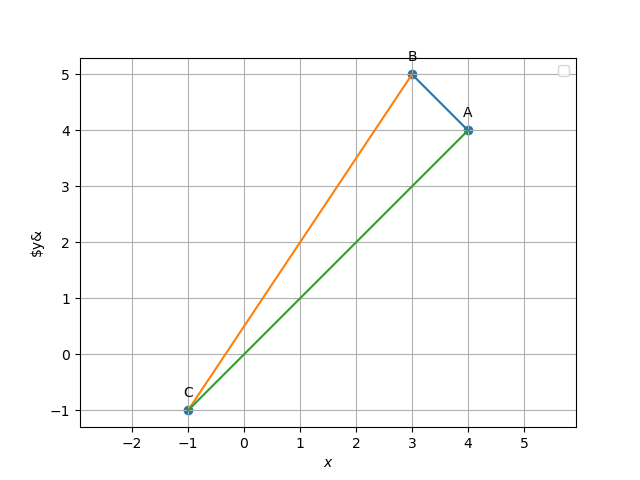
\includegraphics[width=\columnwidth]{chapters/11/10/1/6/figs/triangle.png}
		\caption{}
		\label{fig:11/10/1/6}
  	\end{figure}
